\documentclass{standalone}
\usepackage{tikz}
\usetikzlibrary{arrows.meta}

\begin{document}

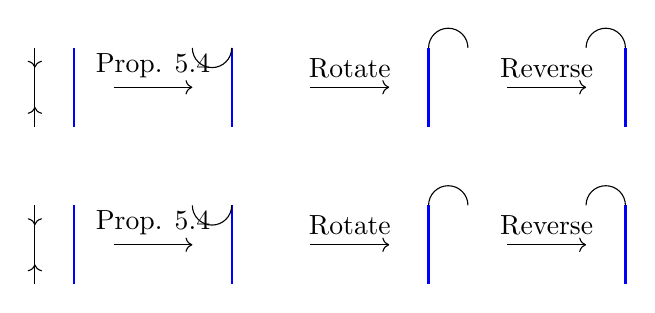
\begin{tikzpicture}[scale=1]

% First Row
% Original Diagram
\foreach \y in {0, -2} {
    % Leftmost diagram
    \draw[blue, thick] (-3, \y+0.5) -- (-3, \y-0.5);
    \draw (-3.5, \y+0.5) -- (-3.5, \y-0.5);
    \draw[->] (-3.5, \y+0.5) -- (-3.5, \y+0.25);
    \draw[->] (-3.5, \y-0.5) -- (-3.5, \y-0.25);

    % Arrow to next diagram
    \draw[->] (-2.5, \y) -- (-1.5, \y) node[midway, above] {Prop. 5.4};

    % Middle diagram
    \draw[blue, thick] (-1, \y+0.5) -- (-1, \y-0.5);
    \draw (-1.5, \y+0.5) arc[start angle=180, end angle=360, radius=0.25];
    
    % Arrow to next diagram
    \draw[->] (0, \y) -- (1, \y) node[midway, above] {Rotate};

    % Rightmost diagram
    \draw[blue, thick] (1.5, \y+0.5) -- (1.5, \y-0.5);
    \draw (2, \y+0.5) arc[start angle=0, end angle=180, radius=0.25];

    % Arrow to final diagram
    \draw[->] (2.5, \y) -- (3.5, \y) node[midway, above] {Reverse};

    % Final diagram
    \draw[blue, thick] (4, \y+0.5) -- (4, \y-0.5);
    \draw (3.5, \y+0.5) arc[start angle=180, end angle=0, radius=0.25];
}

\end{tikzpicture}

\end{document}